\documentclass[12pt,a4paper]{report}

\usepackage{fontspec}
\usepackage[a4paper,left=2.5cm,right=2cm,top=2cm,bottom=2cm]{geometry}
\usepackage{graphicx}
\usepackage{tikz}
\usepackage{longtable}
\usepackage{array}
\usepackage{amsmath}
\usepackage[hidelinks]{hyperref}

\IfFontExistsTF{Times New Roman}{\setmainfont{Times New Roman}}{\setmainfont{Arial}}
\defaultfontfeatures{Ligatures=TeX}
\graphicspath{{figures/}}
\makeatletter
\renewcommand\normalsize{\@setfontsize\normalsize{13pt}{17pt}}
\normalsize
\makeatother
\sloppy

\renewcommand{\contentsname}{Mục lục}
\renewcommand{\listfigurename}{Danh mục hình}
\renewcommand{\listtablename}{Danh mục bảng}
\renewcommand{\bibname}{Tài liệu tham khảo}
\renewcommand{\figurename}{Hình}
\renewcommand{\tablename}{Bảng}
\renewcommand{\chaptername}{Chương}
\setcounter{tocdepth}{1}
\setcounter{secnumdepth}{2}
\newcommand{\placeholder}[1]{\textit{[#1]}}

\begin{document}

\begin{titlepage}
\begin{tikzpicture}[remember picture,overlay,inner sep=0,outer sep=0]
     \draw[blue!70!black,line width=4pt]
     ([xshift=-1.5cm,yshift=-2cm]current page.north east) coordinate (A)
     --([xshift=1.5cm,yshift=-2cm]current page.north west) coordinate(B)
     --([xshift=1.5cm,yshift=2cm]current page.south west) coordinate (C)
     --([xshift=-1.5cm,yshift=2cm]current page.south east) coordinate(D)--cycle;

     \draw ([yshift=0.5cm,xshift=-0.5cm]A)-- ([yshift=0.5cm,xshift=0.5cm]B)--
     ([yshift=-0.5cm,xshift=0.5cm]B) --([yshift=-0.5cm,xshift=-0.5cm]B)
     --([yshift=0.5cm,xshift=-0.5cm]C)--([yshift=0.5cm,xshift=0.5cm]C)
     --([yshift=-0.5cm,xshift=0.5cm]C)-- ([yshift=-0.5cm,xshift=-0.5cm]D)
     --([yshift=0.5cm,xshift=-0.5cm]D)--([yshift=0.5cm,xshift=0.5cm]D)
     --([yshift=-0.5cm,xshift=0.5cm]A)--([yshift=-0.5cm,xshift=-0.5cm]A)
     --([yshift=0.5cm,xshift=-0.5cm]A);

     \draw ([yshift=-0.3cm,xshift=0.3cm]A)-- ([yshift=-0.3cm,xshift=-0.3cm]B)--
     ([yshift=0.3cm,xshift=-0.3cm]B) --([yshift=0.3cm,xshift=0.3cm]B)
     --([yshift=-0.3cm,xshift=0.3cm]C)--([yshift=-0.3cm,xshift=-0.3cm]C)
     --([yshift=0.3cm,xshift=-0.3cm]C)-- ([yshift=0.3cm,xshift=0.3cm]D)
     --([yshift=-0.3cm,xshift=0.3cm]D)--([yshift=-0.3cm,xshift=-0.3cm]D)
     --([yshift=0.3cm,xshift=-0.3cm]A)--([yshift=0.3cm,xshift=0.3cm]A)
     --([yshift=-0.3cm,xshift=0.3cm]A);
\end{tikzpicture}

\begin{center}
\vspace{5pt}
{\fontsize{14pt}{10pt}\selectfont
\textbf{TRƯỜNG ĐẠI HỌC KHOA HỌC TỰ NHIÊN}\\[4pt]
\textbf{Đại Học Quốc Gia Hà Nội}}
\end{center}

\vspace{1.5cm}
\begin{center}

\includegraphics[scale=0.3]{logo.jpg}

\vspace{10pt}
{\fontsize{16pt}{17pt}\selectfont
\textbf{BÁO CÁO CUỐI KỲ}\\[5pt]
\textbf{Học phần: Thị giác máy tính}}
\end{center}

\begin{center}
\vspace{5pt}
{\fontsize{18pt}{20pt}\selectfont
\textbf{TRÍCH XUẤT VÙNG TÒA NHÀ TỪ ẢNH\\
CHỤP TỪ TRÊN CAO (AERIAL IMAGES)}}
\end{center}

\vspace{15pt}
{\fontsize{12pt}{15pt}\selectfont
\textbf{Giảng viên bộ môn: Cao Văn Chung}

\vspace{6pt}
\textbf{Nhóm số : 16}

\vspace{6pt}
\textbf{Thành viên nhóm:}

\vspace{5pt}
\begin{tabbing}
\hspace{0.5cm}\=\hspace{8cm}\=\hspace{3cm}\=\hspace{3cm} \kill
{\itshape\textbf{}}\>
{\itshape\textbf{Họ và tên}}\>{\itshape\textbf{MSSV}}\>{\itshape\textbf{Lớp}}\\
\>\textbf{Nguyễn Huy Sơn}\> \textbf{23001922}\> \textbf{K68A4}\\
\>\textbf{Dương Văn Tài}\> \textbf{23001925}\> \textbf{K68A4}\\
\end{tabbing}}

\vfill
\begin{center}
{\large Hà Nội, tháng 5 năm 2026}
\end{center}
\end{titlepage}

\pagenumbering{roman}
\tableofcontents
\clearpage
\pagenumbering{arabic}

\chapter*{Tóm tắt}
\addcontentsline{toc}{chapter}{Tóm tắt}

Báo cáo này trình bày một quy trình phân đoạn dấu chân công trình (building footprint) từ ảnh hàng không, đặt trong bối cảnh hỗ trợ cập nhật bản đồ đô thị và phân tích sử dụng đất ở mức cơ bản. Dữ liệu ảnh hàng không thường chứa nhiều kiểu mái nhà, đường giao thông, cây xanh, bãi đỗ xe và bóng đổ trong cùng một cảnh. Vì vậy, việc nhận diện vùng công trình không chỉ là bài toán tách màu đơn giản mà còn đòi hỏi đánh giá đồng thời về hình dạng, độ phủ diện tích, số vùng công trình và mức độ nhầm lẫn với các đối tượng nền.

Nghiên cứu sử dụng Inria Aerial Image Labeling Dataset, làm việc với ảnh RGB và mặt nạ nhị phân ground truth. Ảnh gốc được chia ở mức ảnh trước khi cắt thành các patch kích thước 512 $\times$ 512 pixel, nhằm hạn chế rò rỉ dữ liệu giữa tập huấn luyện, tập validation và tập kiểm thử. Bốn hướng tiếp cận được so sánh trên cùng một pipeline: phân cụm K-Means, phân ngưỡng Otsu, Linear SVM với đặc trưng thủ công ở mức pixel, và mạng U-Net cho phân đoạn ngữ nghĩa. Các phương pháp đều được hậu xử lý bằng hình thái học và lọc thành phần liên thông để giảm nhiễu nhỏ.

Kết quả thực nghiệm trên 300 patch kiểm thử cho thấy U-Net đạt kết quả tốt nhất trong nhóm phương pháp đã khảo sát, với IoU trung bình 0.544 và Dice trung bình 0.665. U-Net cũng có sai số diện tích trung bình thấp nhất, khoảng 5.258 điểm phần trăm, và sai số số lượng công trình trung bình 8.217 vùng. SVM cải thiện rõ so với K-Means và Otsu ở IoU/Dice, nhưng vẫn dự đoán thừa diện tích do chỉ phân loại từng pixel dựa trên đặc trưng cục bộ. Otsu có Recall cao nhất trong nhóm baseline nhưng Precision thấp, phản ánh xu hướng gộp nhiều vùng nền sáng thành công trình. Báo cáo đồng thời phân tích các lỗi định tính như false positive ở đường và bãi bê tông, bỏ sót mái nhỏ, ảnh hưởng của bóng đổ và hiện tượng gộp vùng do hậu xử lý.

\chapter*{Mở đầu}
\addcontentsline{toc}{chapter}{Mở đầu}

\section*{Bối cảnh đề tài}

\subsection*{Ảnh hàng không và nhu cầu dữ liệu đô thị}

Ảnh hàng không và ảnh vệ tinh độ phân giải cao là nguồn dữ liệu quan trọng cho hệ thống thông tin địa lý (Geographic Information System, GIS). Tự động trích xuất vùng công trình từ ảnh này giúp cập nhật bản đồ, ước lượng mật độ xây dựng và hỗ trợ theo dõi biến động đô thị.

\subsection*{Bài toán phân đoạn dấu chân công trình}

Dấu chân công trình (building footprint) là vùng chiếm dụng mặt bằng của công trình khi quan sát từ trên cao. Báo cáo mô hình hóa bài toán như phân đoạn nhị phân: đầu vào là patch ảnh RGB, đầu ra là mặt nạ dạng lưới điểm ảnh của vùng công trình. Kết quả được đánh giá bằng mức chồng lấp mask và các thống kê gần với ứng dụng như số vùng công trình, tỷ lệ diện tích.

\section*{Lý do chọn đề tài}

\subsection*{Lý do thực tiễn}

Trong thực tế, dấu chân công trình là lớp dữ liệu nền quan trọng cho quy hoạch đô thị và quản lý hạ tầng. Bài toán cũng đủ thách thức vì mái nhà đa dạng màu, đường hoặc sân bê tông dễ giống công trình, cây xanh che khuất mái và bóng đổ làm thay đổi cường độ sáng.

\subsection*{Lý do khoa học}

Về mặt phương pháp, đề tài so sánh nhiều cấp độ mô hình hóa trong cùng một pipeline: K-Means và Otsu cho nhóm cổ điển, Linear SVM cho học máy có giám sát ở mức pixel, và U-Net cho học sâu. Việc đặt các phương pháp trên cùng dữ liệu, hậu xử lý và bộ chỉ số giúp làm rõ trade-off giữa độ chính xác, tốc độ và tài nguyên tính toán.

\section*{Mục tiêu nghiên cứu}

\subsection*{Mục tiêu tổng quát}

Mục tiêu tổng quát của đề tài là xây dựng và đánh giá một pipeline phân đoạn dấu chân công trình từ ảnh hàng không, bao gồm chuẩn bị dữ liệu, cắt patch, tiền xử lý, dự đoán mặt nạ, hậu xử lý, đánh giá định lượng và trực quan hóa.

\subsection*{Mục tiêu cụ thể}

Các mục tiêu cụ thể gồm: tổ chức dữ liệu để hạn chế rò rỉ giữa các tập; triển khai K-Means và Otsu làm baseline; bổ sung Linear SVM với đặc trưng thủ công; huấn luyện U-Net cho phân đoạn ngữ nghĩa; và đánh giá bằng IoU, Dice, Precision, Recall, F1, sai số số lượng, sai số diện tích và thời gian xử lý.

\section*{Phạm vi nghiên cứu}

\subsection*{Phạm vi dữ liệu}

Báo cáo sử dụng ảnh RGB và mặt nạ ground truth từ Inria Aerial Image Labeling Dataset \cite{maggiori2017inria}. Trong lần chạy hiện có, 180 ảnh gốc được chia thành 126 ảnh huấn luyện, 27 ảnh validation và 27 ảnh kiểm thử; các ảnh này sinh tối đa 1200 patch huấn luyện, 300 patch validation và 300 patch kiểm thử kích thước 512 $\times$ 512 pixel.

\subsection*{Phạm vi phương pháp}

Bốn phương pháp được khảo sát gồm K-Means, Otsu, Linear SVM và U-Net. Báo cáo tập trung vào mặt nạ dạng lưới điểm ảnh và thống kê thành phần liên thông; vector hóa sang đa giác GIS nằm ngoài phạm vi hiện tại.

Ngoài độ chính xác, phạm vi nghiên cứu còn quan tâm đến khả năng giải thích lỗi. Các lỗi như dự đoán nhầm đường thành công trình, bỏ sót mái nhỏ, hoặc gộp nhiều công trình gần nhau có ý nghĩa trực tiếp với ứng dụng bản đồ. Vì vậy, phần kết quả không chỉ trình bày bảng số liệu mà còn có hình chồng lớp định tính.

\chapter{Cơ sở lý thuyết}

\section{Phân đoạn ảnh trong viễn thám}

\subsection{Khái niệm phân đoạn ảnh}

Phân đoạn ảnh là quá trình chia ảnh thành các vùng hoặc nhóm pixel có cùng đặc điểm. Trong phân đoạn ngữ nghĩa, mỗi pixel được gán một nhãn lớp và kết quả là bản đồ nhãn có cùng kích thước với ảnh đầu vào. Với ảnh hàng không, bài toán khó hơn do góc nhìn từ trên cao, mật độ đối tượng lớn, bóng đổ và sự tương đồng màu giữa mái nhà, đường, sân bê tông hoặc cây xanh.

Ảnh viễn thám thường chứa nhiều đối tượng nhỏ, dày đặc và có biên không hoàn toàn rõ. Vì vậy, mô hình phân đoạn cần kết hợp thông tin cục bộ ở mức pixel với ngữ cảnh vùng lân cận để tạo bản đồ nhãn ổn định.

\subsection{Phân đoạn nhị phân}

Phân đoạn nhị phân là trường hợp mỗi pixel thuộc một trong hai lớp: đối tượng quan tâm hoặc nền. Cách biểu diễn này phù hợp khi cần tách riêng vùng công trình, đồng thời thuận tiện cho các chỉ số chồng lấp như giao trên hợp (Intersection over Union, IoU) và hệ số Dice (Dice coefficient). Hạn chế của cách biểu diễn này là toàn bộ nền bị gộp thành một lớp rất đa dạng, làm tăng nguy cơ nhầm lẫn với các bề mặt giống công trình.

\section{Dấu chân công trình trong ảnh hàng không}

\subsection{Khái niệm và biểu diễn}

Dấu chân công trình là hình chiếu hoặc vùng bao phủ của công trình khi quan sát từ trên cao. Trong ảnh hàng không, vùng này thường tương ứng với mái nhà nhưng có thể lệch so với footprint địa lý do góc chụp, bóng đổ hoặc phần nhô mái. Dạng mặt nạ lưới điểm ảnh thuận tiện cho huấn luyện mô hình phân đoạn, còn dạng đa giác phù hợp hơn với GIS; trong pipeline này, mặt nạ lưới điểm ảnh là đầu ra chính.

\subsection{Đặc điểm gây khó trong trích xuất công trình}

Công trình có hình dạng và vật liệu mái rất đa dạng, từ nhà nhỏ độc lập đến khối nhà lớn, từ mái sáng đến mái tối hoặc bị che bởi cây. Các đối tượng nền như đường, vỉa hè, bãi đỗ xe và sân bê tông có thể gần giống mái nhà về màu và độ sáng. Vì vậy, kết quả phân đoạn cần được phân tích cả định lượng lẫn định tính.

\section{Không gian màu và tăng cường ảnh}

\subsection{Không gian màu RGB, HSV và LAB}

RGB là biểu diễn phổ biến của ảnh số nhưng trộn lẫn thông tin màu và độ sáng. HSV tách sắc độ, độ bão hòa và độ sáng, thuận tiện cho phân ngưỡng hoặc phân cụm theo đặc trưng màu. LAB tách kênh độ sáng khỏi hai kênh màu đối lập, nên phù hợp cho các thao tác tăng cường tương phản mà hạn chế làm biến dạng màu.

Việc chuyển đổi không gian màu không tự tạo ra thông tin mới, nhưng có thể làm cho một số đặc trưng trở nên dễ tách hơn. Ví dụ, kênh độ sáng có thể dùng cho tăng tương phản, còn kênh độ bão hòa có thể hỗ trợ phân biệt một số vùng nền và mái. Trong thực nghiệm, các không gian màu này được dùng như đặc trưng đầu vào cho các phương pháp cổ điển và học máy.

\subsection{CLAHE}

CLAHE là kỹ thuật cân bằng histogram thích nghi có giới hạn tương phản (Contrast Limited Adaptive Histogram Equalization). Ảnh được chia thành các vùng nhỏ, histogram cục bộ được điều chỉnh, sau đó nội suy để tránh ranh giới gắt. Kỹ thuật này giúp làm rõ biên và vùng tương phản thấp, nhưng cũng có thể làm nổi bật nhiễu nếu nền có kết cấu giống công trình.

\section{Phân ngưỡng Otsu}

\subsection{Nguyên lý}

Phân ngưỡng chuyển ảnh xám hoặc một kênh đặc trưng thành ảnh nhị phân. Otsu tự động chọn ngưỡng bằng cách tối đa hóa phương sai giữa hai lớp pixel \cite{otsu1979threshold}. Khi histogram có hai nhóm rõ, phương pháp này tách đối tượng và nền với chi phí tính toán thấp.

\subsection{Ưu điểm và hạn chế}

Otsu đơn giản, nhanh và không cần dữ liệu huấn luyện, nên phù hợp làm baseline. Hạn chế chính là giả định một ngưỡng toàn cục đủ tách hai lớp. Trong ảnh hàng không, ánh sáng, bóng đổ và vật liệu bề mặt làm histogram phức tạp; Otsu cũng không khai thác hình dạng hoặc ngữ cảnh không gian.

Về mặt toán học, với histogram chuẩn hóa $p_i$ trên $L$ mức xám, một ngưỡng $t$ chia ảnh thành hai lớp có xác suất:
\[
\omega_0(t)=\sum_{i=0}^{t}p_i,\qquad
\omega_1(t)=\sum_{i=t+1}^{L-1}p_i.
\]
Gọi $\mu_0(t)$ và $\mu_1(t)$ là trung bình cường độ của hai lớp, Otsu chọn ngưỡng tối ưu bằng cách cực đại hóa phương sai giữa lớp:
\[
t^{*}=\arg\max_t \sigma_B^2(t),\qquad
\sigma_B^2(t)=\omega_0(t)\omega_1(t)\left(\mu_0(t)-\mu_1(t)\right)^2.
\]

\section{Phân cụm K-Means}

\subsection{Nguyên lý}

K-Means là phương pháp học không giám sát dùng để chia dữ liệu thành $K$ cụm dựa trên khoảng cách trong không gian đặc trưng \cite{macqueen1967methods}. Trong phân đoạn ảnh, mỗi pixel được biểu diễn bằng vector đặc trưng màu hoặc cường độ; sau phân cụm, một cụm được ánh xạ thành đối tượng mục tiêu.

\subsection{Ưu điểm và hạn chế}

K-Means dễ triển khai và có thể dùng nhiều kênh đặc trưng hơn phân ngưỡng. Tuy nhiên, kết quả phụ thuộc vào số cụm, chuẩn hóa đặc trưng và quy tắc chọn cụm. Phương pháp cũng chưa mô hình hóa trực tiếp hình dạng công trình.

Với tập điểm đặc trưng $\{x_i\}_{i=1}^{n}$, K-Means tối thiểu hóa tổng bình phương khoảng cách nội cụm:
\[
J=\sum_{k=1}^{K}\sum_{x_i\in C_k}\left\|x_i-\mu_k\right\|^2.
\]
Hai bước chính được lặp đến khi hội tụ: gán cụm $c_i=\arg\min_k \|x_i-\mu_k\|^2$ và cập nhật tâm cụm
\[
\mu_k=\frac{1}{|C_k|}\sum_{x_i\in C_k}x_i.
\]

\section{Support Vector Machine}

\subsection{Khái niệm}

Support Vector Machine (SVM) là mô hình học có giám sát dùng cho phân loại và hồi quy. Trong phân loại tuyến tính, SVM tìm siêu phẳng phân tách hai lớp với biên lớn nhất \cite{cortes1995support}. Tham số $C$ điều khiển mức phạt cho lỗi phân loại trong trường hợp dữ liệu không tách hoàn hảo.

\subsection{SVM trong phân đoạn mức pixel}

Khi áp dụng cho phân đoạn, mỗi pixel được xem như một mẫu huấn luyện với nhãn công trình hoặc nền. Vector đặc trưng có thể gồm màu, độ sáng, gradient và thống kê cục bộ. SVM tận dụng được nhãn, nhưng vẫn thiếu ngữ cảnh không gian rộng nên dễ nhầm các bề mặt có đặc trưng cục bộ giống mái nhà.

\section{Mạng U-Net}

\subsection{Kiến trúc encoder-decoder}

U-Net là kiến trúc mạng tích chập phổ biến cho phân đoạn ảnh, gồm encoder, decoder và skip connection \cite{ronneberger2015unet}. Encoder học đặc trưng ngữ cảnh ở độ phân giải thấp, decoder khôi phục bản đồ phân đoạn, còn skip connection giúp giữ chi tiết biên.

\subsection{Ý nghĩa trong phân đoạn công trình}

Đối với ảnh hàng không, U-Net có thể học hình dạng, kết cấu và ngữ cảnh của công trình thay vì chỉ dựa vào màu từng pixel. Đổi lại, mô hình cần dữ liệu gán nhãn, thời gian huấn luyện và khả năng kiểm soát overfitting.

Ưu điểm của skip connection trong U-Net là giúp decoder khôi phục chi tiết biên tốt hơn so với encoder-decoder thuần túy. Điều này quan trọng với building footprint vì biên công trình quyết định trực tiếp IoU, Dice và khả năng sử dụng mặt nạ cho bước vector hóa sau này.

\section{Hậu xử lý hình thái học}

\subsection{Closing, opening và lọc thành phần liên thông}

Hậu xử lý hình thái học giúp cải thiện mặt nạ nhị phân sau phân đoạn. Closing lấp lỗ nhỏ và nối vùng đứt đoạn; opening loại nhiễu nhỏ; phân tích thành phần liên thông dùng để lọc vùng nhỏ và đếm số vùng công trình.

\subsection{Tác động hai mặt}

Hậu xử lý làm mặt nạ ổn định hơn nhưng có thể loại bỏ công trình nhỏ, gộp công trình gần nhau hoặc làm biến dạng biên. Vì vậy, cần đánh giá tác động của nó cùng với kết quả định lượng và trực quan.

\section{Chỉ số đánh giá}

\subsection{IoU và Dice}

Giao trên hợp (Intersection over Union, IoU) đo tỷ lệ giữa phần giao của mặt nạ dự đoán và ground truth so với phần hợp:
\[
\mathrm{IoU} = \frac{TP}{TP + FP + FN}.
\]
Hệ số Dice đo mức chồng lấp theo công thức:
\[
\mathrm{Dice} = \frac{2TP}{2TP + FP + FN}.
\]
Hai chỉ số này phản ánh chất lượng chồng lấp không gian của mặt nạ.

\subsection{Precision, Recall và F1}

Precision đo tỷ lệ pixel dự đoán là công trình thật sự thuộc công trình:
\[
\mathrm{Precision} = \frac{TP}{TP + FP}.
\]
Recall đo tỷ lệ pixel công trình thật được phát hiện:
\[
\mathrm{Recall} = \frac{TP}{TP + FN}.
\]
F1 là trung bình điều hòa giữa Precision và Recall. Precision thấp thường thể hiện dự đoán thừa nền thành công trình; Recall thấp thể hiện bỏ sót công trình.

\subsection{Sai số số lượng và sai số diện tích}

Bên cạnh chỉ số pixel-level, bài toán địa không gian cần quan tâm đến số vùng công trình và tỷ lệ diện tích xây dựng. Sai số số lượng phản ánh chênh lệch số thành phần liên thông; sai số diện tích phản ánh chênh lệch tỷ lệ pixel công trình. Hai chỉ số này giúp đánh giá gần hơn với nhu cầu ứng dụng bản đồ.

Một mô hình có Dice tương đối tốt vẫn có thể chưa phù hợp nếu gộp nhiều nhà gần nhau thành một vùng hoặc dự đoán sai tổng diện tích xây dựng. Vì vậy, việc kết hợp chỉ số pixel-level với thống kê vùng giúp đánh giá kết quả cân bằng hơn giữa mục tiêu học máy và mục tiêu ứng dụng GIS.

\chapter{Phương pháp nghiên cứu}

\section{Tổng quan pipeline thực nghiệm}

Pipeline thực nghiệm được thiết kế theo chuỗi xử lý từ dữ liệu ảnh đến kết quả định lượng. Hệ thống đọc ảnh RGB và mặt nạ từ Inria Aerial Image Labeling Dataset, chia ảnh gốc thành train/validation/test, sau đó cắt thành patch 512 $\times$ 512 pixel. Mỗi patch được tiền xử lý bằng CLAHE trên kênh sáng LAB rồi đưa vào bốn nhánh mô hình: K-Means, Otsu, Linear SVM và U-Net. Mặt nạ dự đoán được hậu xử lý bằng closing, opening và lọc thành phần liên thông trước khi tính IoU, Dice, Precision, Recall, F1, count error, area error và thời gian xử lý.

Điểm quan trọng của pipeline là mọi phương pháp được đánh giá trên cùng test set và cùng bước hậu xử lý. Thiết kế này giúp so sánh tập trung vào khác biệt giữa chiến lược phân đoạn, thay vì bị nhiễu bởi khác biệt về dữ liệu hoặc cách tính chỉ số. Các sản phẩm đầu ra gồm tệp CSV chỉ số, hình so sánh phương pháp, ảnh chồng lớp định tính và checkpoint mô hình.

\section{Dữ liệu và chia tập}

\subsection{Bộ dữ liệu}

Dữ liệu sử dụng là Inria Aerial Image Labeling Dataset, một bộ dữ liệu chuẩn ảnh hàng không độ phân giải cao cho bài toán gán nhãn vùng công trình \cite{maggiori2017inria}. Danh sách dữ liệu hiện có năm khu vực: Austin, Chicago, Kitsap, Tyrol-w và Vienna. Bộ dữ liệu cung cấp cả ảnh RGB và mặt nạ nhị phân ground truth, cho phép đánh giá bằng IoU, Dice và các chỉ số pixel-level.

\subsection{Chiến lược chia tập}

Ảnh gốc được xáo trộn với seed cố định và chia theo tỷ lệ 70\% train, 15\% validation và 15\% test. Danh sách dữ liệu gồm 126 ảnh train, 27 ảnh validation và 27 ảnh test, sinh tối đa 1200/300/300 patch tương ứng. Cách chia ở mức ảnh gốc giúp hạn chế rò rỉ dữ liệu giữa các tập.

Việc giới hạn số patch là lựa chọn thực dụng để cân bằng giữa độ phủ dữ liệu và tài nguyên tính toán. Với Inria, một ảnh gốc có thể sinh nhiều patch, nhưng việc dùng toàn bộ patch sẽ làm tăng thời gian huấn luyện U-Net và tuning SVM. Do đó, số patch được giới hạn nhưng vẫn giữ đủ mẫu cho đánh giá định lượng trên test set.

\begin{table}[htbp]
\centering
\caption{Quy mô dữ liệu trong danh sách thực nghiệm}
\label{tab:data-split}
\begin{tabular}{|l|r|r|p{6.8cm}|}
\hline
\textbf{Split} & \textbf{Số ảnh gốc} & \textbf{Số patch} & \textbf{Thành phố}\\
\hline
Train & 126 & 1200 & Austin, Chicago, Kitsap, Tyrol-w, Vienna\\
\hline
Validation & 27 & 300 & Austin, Chicago, Kitsap, Tyrol-w, Vienna\\
\hline
Test & 27 & 300 & Austin, Chicago, Kitsap, Tyrol-w, Vienna\\
\hline
\end{tabular}
\end{table}

\section{Tiền xử lý ảnh}

Mỗi patch được chuyển từ RGB sang LAB, áp dụng CLAHE trên kênh sáng với clip limit 2.0 và lưới 8 $\times$ 8, sau đó chuyển ngược về RGB. Bước này làm rõ tương phản cục bộ và được dùng nhất quán cho các nhánh chính để bảo đảm so sánh công bằng.

Trong ảnh hàng không, các vùng mái có thể nằm dưới bóng cây hoặc có độ tương phản thấp so với nền xung quanh. CLAHE giúp tăng khả năng quan sát chi tiết cục bộ, nhưng không thay thế mô hình phân đoạn. Vì vậy, tiền xử lý được xem là bước chuẩn hóa đầu vào trước khi so sánh các thuật toán.

\section{Phân đoạn bằng K-Means}

Nhánh K-Means dùng đặc trưng RGB và HSV của từng pixel, chuẩn hóa về miền số thực rồi phân cụm với $K=4$. Cụm có giá trị trung tâm cao nhất trên kênh độ sáng HSV được chọn làm ứng viên công trình. Đây là baseline không giám sát, nhưng quy tắc chọn cụm theo độ sáng dễ sinh false positive ở đường, bãi bê tông hoặc vùng nền sáng.

Kết quả của nhánh này sau đó được đưa qua morphology như các phương pháp khác. Việc giữ cùng hậu xử lý giúp kiểm tra xem bản thân phân cụm màu có tạo được mặt nạ đủ tốt hay không, thay vì để nhiễu nhỏ chi phối toàn bộ kết quả.

\section{Phân đoạn bằng Otsu}

Nhánh Otsu chuyển patch sang HSV, lấy kênh độ bão hòa, áp dụng CLAHE nhẹ với clip limit 1.5 rồi tìm ngưỡng tự động. Đây là baseline nhanh, nhưng do chỉ dựa trên một kênh đặc trưng và một ngưỡng toàn cục nên dễ dự đoán quá rộng khi nền có độ bão hòa tương tự công trình.

Otsu được giữ trong thực nghiệm vì nó thể hiện rõ giới hạn của phương pháp thresholding trong ảnh đô thị. Khi so sánh với K-Means, SVM và U-Net, kết quả Otsu giúp làm nổi bật giá trị của đặc trưng đa kênh, nhãn huấn luyện và ngữ cảnh không gian.

\section{Phân đoạn bằng Linear SVM}

\subsection{Đặc trưng pixel}

Nhánh SVM trích xuất vector đặc trưng cho từng pixel từ patch đã tiền xử lý, gồm RGB, LAB, HSV, grayscale, độ lớn gradient Sobel, trung bình cục bộ và độ lệch chuẩn cục bộ. Nhờ vậy, mô hình khai thác cả màu, biên và kết cấu lân cận.

\subsection{Lấy mẫu và huấn luyện}

Từ mỗi patch train, pipeline lấy tối đa 1200 pixel và giới hạn tổng số pixel huấn luyện ở 200000. Mô hình dùng StandardScaler và LinearSVC với class weight cân bằng, max iteration 5000 và thử $C \in \{0.1,0.5,1.0\}$ trên validation set. Mô hình có Dice validation cao nhất được lưu để đánh giá trên test set.

SVM đóng vai trò cầu nối giữa baseline truyền thống và học sâu. Nó khai thác ground truth ở mức pixel, nhưng vẫn phụ thuộc vào đặc trưng thủ công và ranh giới tuyến tính. Do đó, phương pháp này giúp đánh giá phần cải thiện đến từ học có giám sát trước khi chuyển sang U-Net.

\section{Phân đoạn bằng U-Net}

\subsection{Chuẩn bị dữ liệu}

Đối với U-Net, mỗi mẫu gồm một patch ảnh đã tiền xử lý và mặt nạ ground truth tương ứng. Ảnh được chuẩn hóa về miền [0, 1]. Trong huấn luyện, pipeline dùng lật ngang, lật dọc, xoay theo bội số 90 độ, thay đổi nhẹ độ sáng và độ tương phản.

\subsection{Kiến trúc}

U-Net trong thực nghiệm là phiên bản nhỏ gồm ba mức encoder, một bridge và ba mức decoder. Các khối chính dùng convolution 3 $\times$ 3, batch normalization và ReLU; decoder dùng transposed convolution và skip connection. Lớp đầu ra là convolution 1 $\times$ 1 tạo logit một kênh cho phân đoạn nhị phân.

\subsection{Huấn luyện và chọn ngưỡng}

Mô hình được huấn luyện tối đa 20 epoch, batch size 4, learning rate $10^{-3}$, suy giảm trọng số $10^{-4}$ và optimizer AdamW. Hàm mất mát là tổng của BCEWithLogitsLoss và Dice loss. Sau huấn luyện, các ngưỡng 0.3, 0.4, 0.5, 0.6 và 0.7 được thử trên validation set; ngưỡng 0.4 đạt Dice validation cao nhất.

Việc chọn ngưỡng trên validation set là cần thiết vì xác suất đầu ra của U-Net không nhất thiết tối ưu tại 0.5. Ngưỡng thấp hơn có thể tăng Recall, trong khi ngưỡng cao hơn thường tăng Precision. Chọn theo Dice giúp cân bằng hai xu hướng này trước khi đánh giá test.

\section{Hậu xử lý và đánh giá}

Tất cả mặt nạ dự đoán được đưa qua closing 9 $\times$ 9, opening 5 $\times$ 5 và lọc thành phần liên thông nhỏ hơn 200 pixel. Đánh giá được thực hiện trên từng patch test bằng IoU, Dice, Precision, Recall, F1, số vùng dự đoán, số vùng ground truth, sai số số lượng, sai số diện tích và thời gian dự đoán.

\section{Cấu hình thực nghiệm}

\begin{table}[htbp]
\centering
\caption{Cấu hình chính của pipeline}
\label{tab:config}
\small
\begin{tabular}{|p{5.2cm}|p{8.8cm}|}
\hline
\textbf{Nhóm cấu hình} & \textbf{Giá trị}\\
\hline
Patch & Size 512 $\times$ 512, stride 512\\
\hline
Split & Train/validation/test = 70\%/15\%/15\%\\
\hline
Giới hạn patch & Train 1200, validation 300, test 300\\
\hline
CLAHE & Clip limit 2.0, lưới ô 8 $\times$ 8\\
\hline
K-Means & $K=4$, max iteration 10, epsilon 1.0, 3 lần khởi tạo\\
\hline
Otsu & CLAHE trên kênh độ bão hòa với clip limit 1.5\\
\hline
SVM & LinearSVC, trọng số lớp cân bằng, $C \in \{0.1,0.5,1.0\}$, tối đa 200000 pixel huấn luyện\\
\hline
U-Net & 20 epoch, batch size 4, learning rate $10^{-3}$, suy giảm trọng số $10^{-4}$, patience 5\\
\hline
Hậu xử lý & Closing 9 $\times$ 9, opening 5 $\times$ 5, minimum area 200 pixel\\
\hline
\end{tabular}
\end{table}

\chapter{Thực nghiệm và kết quả}

\section{Kết quả định lượng tổng hợp}

\subsection{Bảng kết quả chính}

Bảng \ref{tab:main-results} trình bày kết quả trung bình trên 300 patch kiểm thử. Các chỉ số IoU, Dice, Precision, Recall và F1 nằm trong miền [0, 1], càng cao càng tốt. Count Error, Area Error và Seconds/Patch càng thấp càng tốt. Area Error được tính theo điểm phần trăm diện tích patch.

\begin{table}[htbp]
\centering
\caption{So sánh định lượng các phương pháp trên tập test}
\label{tab:main-results}
\small
\setlength{\tabcolsep}{3pt}
\renewcommand{\arraystretch}{1.15}
\begin{tabular}{|l|r|r|r|r|r|r|r|r|}
\hline
\textbf{Phương pháp} & \textbf{IoU} & \textbf{Dice} & \textbf{Prec.} & \textbf{Recall} & \textbf{F1} & \textbf{Count Err.} & \textbf{Area Err.} & \textbf{s/patch}\\
\hline
K-Means & 0.230 & 0.347 & 0.347 & 0.469 & 0.347 & 15.600 & 20.093 & 0.0828\\
\hline
Otsu & 0.223 & 0.333 & 0.233 & 0.802 & 0.333 & 15.037 & 64.691 & 0.0075\\
\hline
SVM & 0.295 & 0.416 & 0.315 & 0.774 & 0.416 & 16.293 & 34.436 & 0.0565\\
\hline
U-Net & 0.544 & 0.665 & 0.698 & 0.673 & 0.665 & 8.217 & 5.258 & 0.0396\\
\hline
\end{tabular}
\end{table}

Kết quả cho thấy U-Net vượt trội rõ rệt ở hai chỉ số chồng lấp chính. IoU trung bình của U-Net đạt 0.544, cao hơn SVM khoảng 0.249 điểm tuyệt đối và cao hơn K-Means/Otsu hơn 0.31 điểm. Dice trung bình của U-Net đạt 0.665, trong khi SVM đạt 0.416, K-Means đạt 0.347 và Otsu đạt 0.333. Điều này cho thấy mô hình học sâu khai thác tốt hơn cấu trúc không gian và hình dạng công trình so với các phương pháp dựa chủ yếu vào đặc trưng màu hoặc pixel độc lập.

Về Precision và Recall, U-Net có Precision cao nhất với 0.698 và Recall 0.673. Otsu và SVM có Recall cao lần lượt 0.802 và 0.774, nhưng Precision thấp hơn nhiều. Mẫu hình này cho thấy Otsu và SVM có xu hướng dự đoán rộng, phát hiện được nhiều pixel công trình thật nhưng đồng thời gán nhầm nhiều nền thành công trình. K-Means có Precision tương đương Dice nhưng Recall chỉ 0.469, phản ánh việc vừa bỏ sót vừa dự đoán nhầm trong các vùng có màu phức tạp.

\subsection{Sai số số lượng và sai số diện tích}

Trong ứng dụng bản đồ, một mặt nạ có Dice cao chưa chắc đã đủ nếu nó gộp nhiều công trình hoặc dự đoán sai tổng diện tích xây dựng. U-Net ổn định nhất với Count Error trung bình 8.217 và Area Error 5.258; tỷ lệ diện tích ground truth trung bình là 22.527\%, trong khi U-Net dự đoán 21.268\%. Ngược lại, Otsu dự đoán tới 87.218\% diện tích patch là công trình, phù hợp với Recall cao nhưng Precision thấp.

\subsection{Thời gian xử lý}

Otsu là phương pháp nhanh nhất với khoảng 0.0075 giây mỗi patch. U-Net đạt khoảng 0.0396 giây mỗi patch trong điều kiện có CUDA cho mô hình, nhanh hơn SVM và K-Means trong lần đo hiện tại. SVM mất khoảng 0.0565 giây mỗi patch do cần trích xuất đặc trưng và phân loại từng pixel. K-Means mất khoảng 0.0828 giây mỗi patch do phải chạy phân cụm trên toàn bộ pixel của patch.

Cần diễn giải thời gian xử lý một cách thận trọng. Với U-Net, bảng chỉ phản ánh thời gian suy luận trên patch test sau khi đã huấn luyện, chưa tính chi phí huấn luyện. Với K-Means và Otsu, gần như không có chi phí huấn luyện. Vì vậy, nếu ứng dụng cần chạy một lần trên tập nhỏ, baseline truyền thống có lợi thế về đơn giản. Nếu ứng dụng cần xử lý nhiều ảnh sau khi đã huấn luyện, U-Net có thể hấp dẫn hơn nhờ chất lượng mặt nạ và tốc độ suy luận tốt trên GPU.

\section{Kết quả tuning}

\subsection{Tuning Linear SVM}

Bảng \ref{tab:svm-tuning} trình bày kết quả thử ba giá trị $C$ cho Linear SVM. Sự khác biệt Dice validation giữa các giá trị rất nhỏ, nhưng $C=0.5$ đạt kết quả cao nhất trong lần chạy này. Điều đó cho thấy trong cấu hình đặc trưng hiện tại, hiệu quả của SVM bị giới hạn nhiều hơn bởi đặc trưng pixel và giả định tuyến tính hơn là bởi lựa chọn $C$ trong khoảng thử hẹp.

\begin{table}[htbp]
\centering
\caption{Kết quả tuning tham số $C$ của SVM}
\label{tab:svm-tuning}
\begin{tabular}{|r|r|r|}
\hline
\textbf{$C$} & \textbf{Validation Dice} & \textbf{Train seconds}\\
\hline
0.1 & 0.2849 & 1.683\\
\hline
0.5 & 0.2851 & 1.407\\
\hline
1.0 & 0.2851 & 1.470\\
\hline
\end{tabular}
\end{table}

\subsection{Tuning ngưỡng U-Net}

U-Net sinh xác suất hoặc logit cho từng pixel, do đó cần chọn ngưỡng để chuyển sang mặt nạ nhị phân. Bảng \ref{tab:unet-threshold} cho thấy ngưỡng 0.4 đạt Dice validation cao nhất, 0.6085. Các ngưỡng 0.5 và 0.6 cho kết quả gần nhau nhưng thấp hơn. Việc ngưỡng tốt nhất nhỏ hơn 0.5 cho thấy mô hình có thể hơi bảo thủ nếu dùng ngưỡng mặc định, và việc hạ ngưỡng giúp tăng phát hiện vùng công trình trên validation set.

\begin{table}[htbp]
\centering
\caption{Kết quả tuning ngưỡng nhị phân hóa U-Net}
\label{tab:unet-threshold}
\begin{tabular}{|r|r|}
\hline
\textbf{Threshold} & \textbf{Validation Dice}\\
\hline
0.3 & 0.5967\\
\hline
0.4 & 0.6085\\
\hline
0.5 & 0.6058\\
\hline
0.6 & 0.6041\\
\hline
0.7 & 0.5929\\
\hline
\end{tabular}
\end{table}

\subsection{Diễn biến huấn luyện U-Net}

U-Net được huấn luyện đủ 20 epoch trong lần chạy hiện tại. Validation loss tốt nhất xuất hiện ở epoch 17, đạt 0.6824. Sau đó loss validation tăng nhẹ ở epoch 18 và giảm lại ở epoch 19, nhưng không vượt qua mốc tốt nhất. Điều này cho thấy mô hình vẫn học được đặc trưng hữu ích trong suốt quá trình huấn luyện, đồng thời bắt đầu có dao động validation ở các epoch cuối.

\begin{table}[htbp]
\centering
\caption{Một số mốc loss trong quá trình huấn luyện U-Net}
\label{tab:unet-training}
\begin{tabular}{|r|r|r|l|}
\hline
\textbf{Epoch} & \textbf{Train loss} & \textbf{Val loss} & \textbf{Thiết bị}\\
\hline
1 & 1.1362 & 1.1292 & cuda\\
\hline
8 & 0.8628 & 0.7906 & cuda\\
\hline
10 & 0.8250 & 0.7265 & cuda\\
\hline
15 & 0.7487 & 0.7062 & cuda\\
\hline
17 & 0.7473 & 0.6824 & cuda\\
\hline
20 & 0.7174 & 0.6939 & cuda\\
\hline
\end{tabular}
\end{table}

\section{Kết quả trực quan}

\begin{figure}[htbp]
\centering

\includegraphics[width=\textwidth]{method_comparison.png}
\caption{Biểu đồ so sánh IoU, Dice, Precision, Recall và F1 của bốn phương pháp}
\label{fig:method-comparison}
\end{figure}

Hình \ref{fig:method-comparison} trực quan hóa sự khác biệt giữa các phương pháp. U-Net có các cột IoU, Dice, Precision và F1 cao nhất. Otsu nổi bật ở Recall nhưng thấp ở Precision, đúng với nhận xét rằng phương pháp này dự đoán quá nhiều pixel công trình. SVM có Recall cao nhưng Precision thấp hơn K-Means, cho thấy mô hình nhận được nhiều vùng công trình hơn nhưng cũng kéo theo nhiều false positive. K-Means có kết quả cân bằng hơn Otsu nhưng mức chồng lấp vẫn thấp.

\begin{figure}[htbp]
\centering
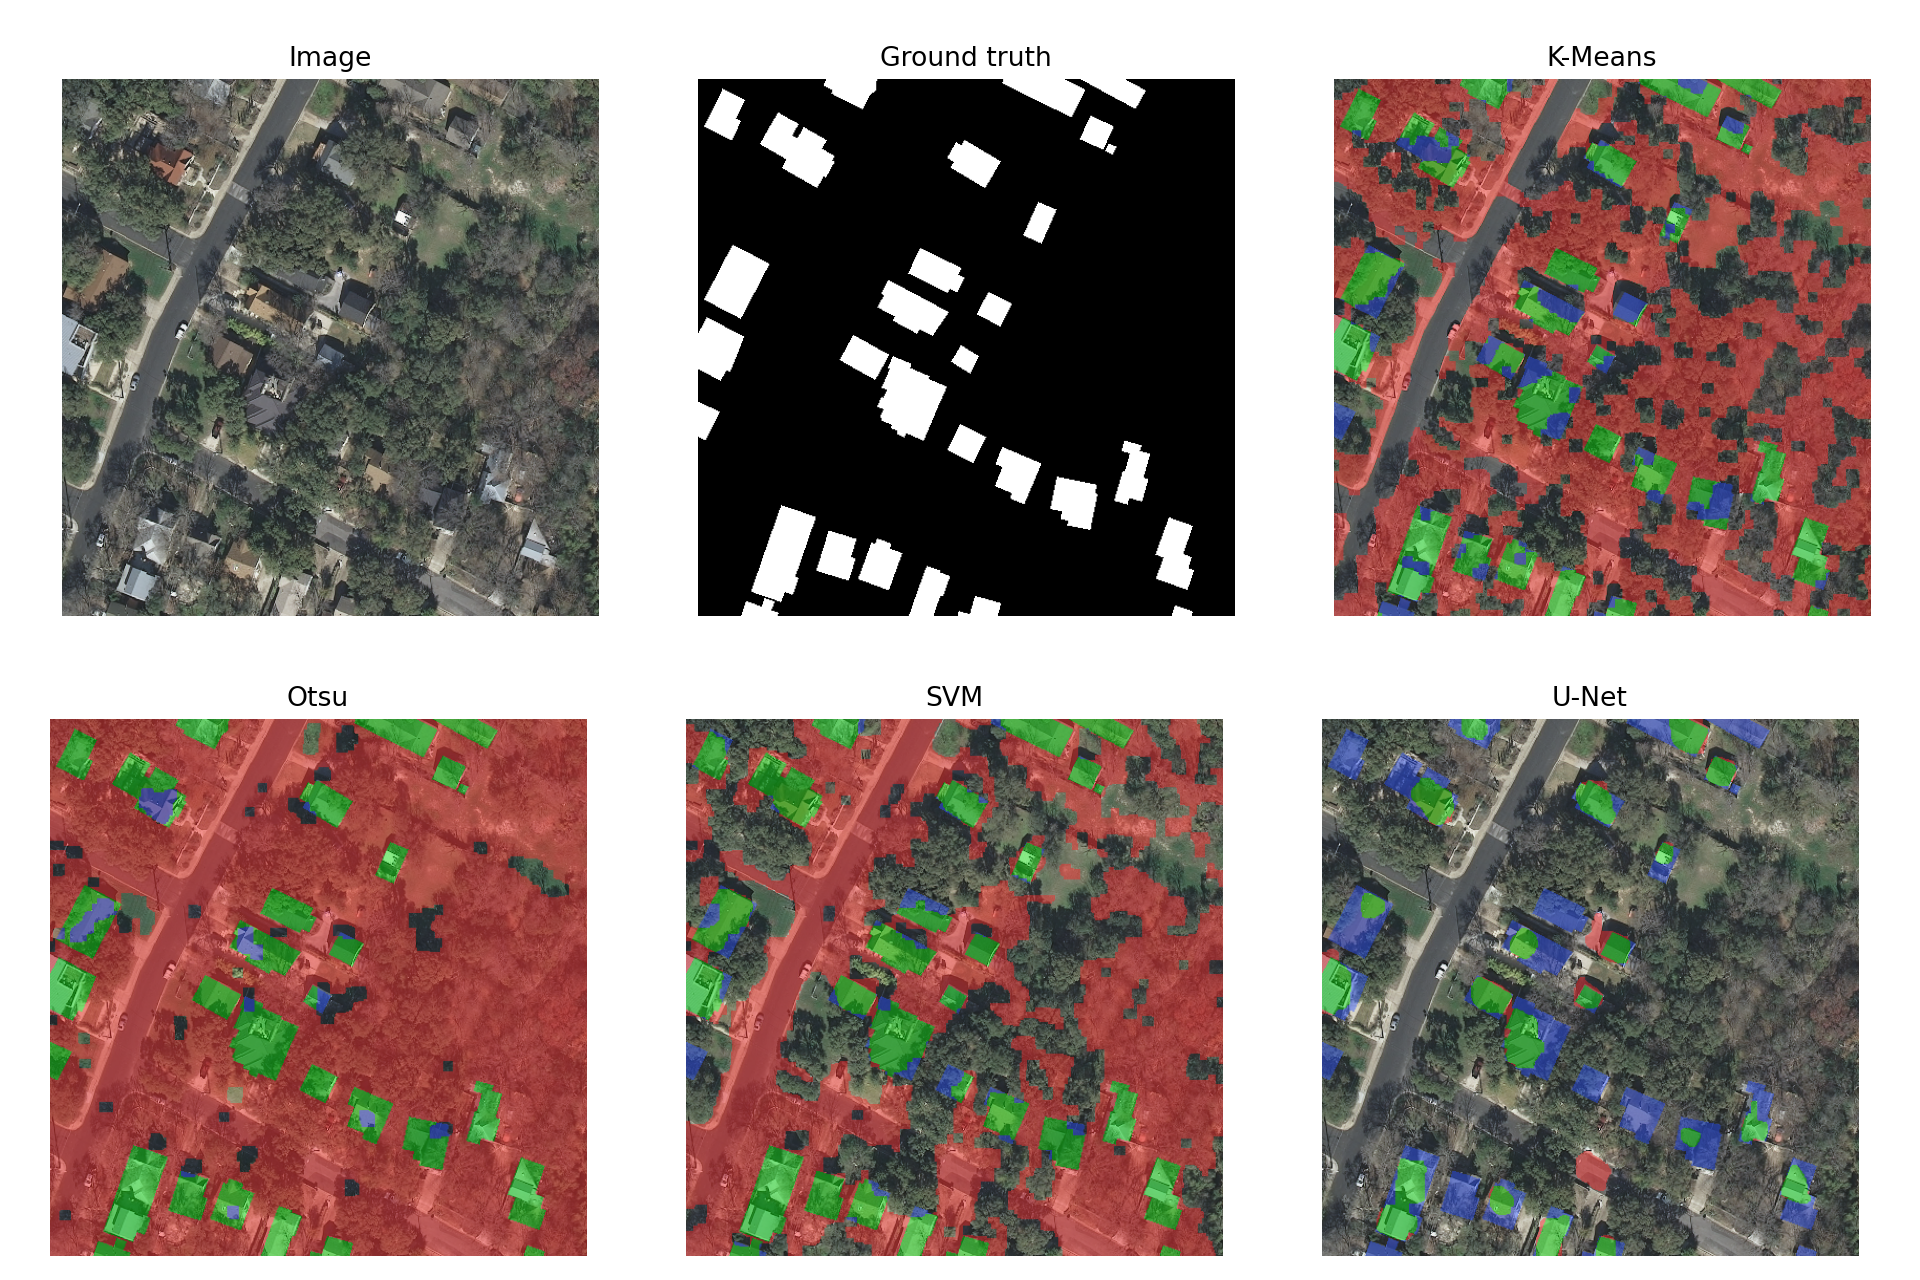
\includegraphics[width=\textwidth]{qualitative_grid_000_2x3.png}
\caption{Ví dụ định tính trên patch test: xanh lá là true positive, đỏ là false positive, xanh dương là false negative}
\label{fig:qualitative-000}
\end{figure}

Hình \ref{fig:qualitative-000} được bố trí thành hai hàng và ba cột để dễ quan sát từng lớp kết quả. K-Means, Otsu và SVM có nhiều vùng đỏ, tức dự đoán nhầm nền thành công trình; U-Net giữ được nhiều vùng mái đúng hơn nhưng vẫn bỏ sót một số công trình nhỏ hoặc vùng bị che khuất.

\section{Phân tích từng phương pháp}

\subsection{K-Means}

K-Means đạt IoU 0.230 và Dice 0.347, cao hơn Otsu một chút nhưng thấp hơn SVM và U-Net. Phương pháp này dự đoán diện tích công trình trung bình 34.400\%, cao hơn ground truth 22.527\%, cho thấy quy tắc chọn cụm sáng dễ bắt thêm đường, sân bê tông hoặc vùng nền sáng.

\subsection{Otsu}

Otsu có IoU 0.223 và Dice 0.333, nhưng Recall đạt 0.802 trong khi Precision chỉ 0.233. Điều này cho thấy phương pháp ít bỏ sót pixel công trình hơn nhưng dự đoán thừa nghiêm trọng; dù rất nhanh với 0.0075 giây mỗi patch, mặt nạ Otsu khó dùng trực tiếp cho bản đồ.

\subsection{Linear SVM}

SVM đạt IoU 0.295 và Dice 0.416, cải thiện rõ so với K-Means và Otsu nhờ dùng RGB, LAB, HSV, gradient và thống kê cục bộ. Tuy nhiên, Precision 0.315 và Area Error 34.436 cho thấy SVM vẫn dự đoán thừa nhiều nền do phân loại từng pixel bằng đặc trưng cục bộ và ranh giới tuyến tính.

\subsection{U-Net}

U-Net đạt kết quả tốt nhất với IoU 0.544, Dice 0.665, Precision 0.698 và Area Error 5.258. Kết quả này cho thấy mô hình học sâu khai thác tốt hơn ngữ cảnh không gian và hình dạng mái, dù vẫn có thể bỏ sót công trình nhỏ, vùng bị che khuất hoặc mái quá tối.

\section{Phân tích lỗi}

\subsection{False positive}

False positive xuất hiện khi nền được dự đoán thành công trình. Các nguồn false positive chính gồm đường bê tông, sân, bãi đỗ xe, vùng đất sáng màu và các mảng cây có kết cấu mạnh. Otsu và SVM chịu ảnh hưởng rõ nhất vì hai phương pháp này có Recall cao nhưng Precision thấp. K-Means cũng sinh false positive khi cụm sáng chứa cả mái và nền. U-Net giảm đáng kể false positive nhưng vẫn có thể nhầm ở vùng có vật liệu giống mái hoặc biên không rõ.

\subsection{False negative}

False negative xuất hiện khi công trình thật bị bỏ sót. Các công trình nhỏ, mái bị cây che, mái tối nằm trong bóng đổ hoặc vùng mái có màu gần giống nền thường là nguồn lỗi chính. U-Net có Precision cao hơn nhưng vẫn bỏ sót một số vùng nhỏ, đặc biệt khi ngưỡng nhị phân hóa hoặc hậu xử lý loại bỏ connected component nhỏ. Điều này cho thấy minimum area 200 pixel là tham số cần cân nhắc nếu ứng dụng quan tâm đến nhà nhỏ.

\subsection{Lỗi gộp và lỗi tách vùng}

Count Error phản ánh khả năng tách/gộp các vùng công trình. Một mặt nạ có thể bao phủ đúng diện tích tổng thể nhưng vẫn gộp nhiều nhà gần nhau thành một vùng hoặc chia một mái nhà thành nhiều mảnh. Closing giúp nối vùng bị đứt đoạn nhưng cũng có thể gộp công trình gần nhau. Opening và lọc diện tích giúp giảm nhiễu nhưng có thể loại công trình nhỏ. Do đó, hậu xử lý cần được điều chỉnh theo mục tiêu: nếu cần thống kê diện tích tổng, tham số có thể khác với trường hợp cần đếm từng tòa nhà.

\section{Thảo luận}

\subsection{Ý nghĩa của kết quả}

Kết quả thực nghiệm xác nhận xu hướng thường gặp trong phân đoạn ảnh hàng không: phương pháp học sâu có lợi thế khi có dữ liệu gán nhãn và tài nguyên tính toán, còn baseline truyền thống hữu ích để hiểu bài toán và tạo điểm so sánh. U-Net không chỉ cải thiện IoU/Dice mà còn đưa tỷ lệ diện tích dự đoán gần với ground truth, điều quan trọng trong ứng dụng ước lượng diện tích xây dựng.

SVM là bước trung gian có giá trị. Nó cho thấy việc thêm nhãn và đặc trưng thủ công cải thiện đáng kể so với K-Means/Otsu, nhưng vẫn chưa đủ để xử lý hoàn toàn sự phức tạp của ảnh đô thị. Điều này củng cố nhận định rằng bài toán dấu chân công trình không chỉ là bài toán màu sắc mà còn là bài toán hình dạng và ngữ cảnh.

\chapter*{Kết luận và hướng phát triển}
\addcontentsline{toc}{chapter}{Kết luận và hướng phát triển}

\section*{Kết luận}

Báo cáo đã trình bày một pipeline phân đoạn dấu chân công trình từ ảnh hàng không, sử dụng Inria Aerial Image Labeling Dataset, chia dữ liệu ở mức ảnh gốc và đánh giá trên patch 512 $\times$ 512 pixel. Bốn phương pháp được so sánh gồm K-Means, Otsu, Linear SVM và U-Net trong cùng quy trình tiền xử lý, hậu xử lý và đánh giá.

Kết quả trên 300 patch test cho thấy U-Net là phương pháp hiệu quả nhất, đạt IoU trung bình 0.544, Dice trung bình 0.665 và sai số diện tích 5.258. SVM cải thiện so với K-Means và Otsu nhưng vẫn dự đoán thừa nhiều vùng nền. Các baseline truyền thống có giá trị tham chiếu, song gặp hạn chế rõ trong cảnh đô thị phức tạp. Việc kết hợp IoU, Dice, Precision, Recall, Count Error, Area Error và phân tích ảnh chồng lớp giúp đánh giá kết quả gần hơn với nhu cầu GIS.

Từ kết quả này có thể rút ra hai nhận xét chính. Thứ nhất, các phương pháp dựa nhiều vào màu hoặc ngưỡng vẫn hữu ích để tạo mốc so sánh nhanh, nhưng khó xử lý ổn định khi nền đô thị có đường, sân bê tông, cây xanh và bóng đổ. Thứ hai, mô hình học sâu có lợi thế rõ hơn vì học được ngữ cảnh không gian và hình dạng công trình, đặc biệt trong các patch có nhiều mái nhà nhỏ hoặc biên phức tạp.

\section*{Hạn chế}

Thực nghiệm còn một số hạn chế. Dữ liệu chỉ sử dụng ảnh RGB và mặt nạ nhị phân, chưa kết hợp độ cao, ảnh đa phổ hoặc siêu dữ liệu địa lý. Những nguồn dữ liệu bổ sung này có thể giúp phân biệt mái nhà với đường, sân bê tông hoặc bãi đỗ xe tốt hơn. Ngoài ra, số patch huấn luyện được giới hạn để phù hợp tài nguyên, nên mô hình chưa khai thác toàn bộ dữ liệu có sẵn.

Về mô hình, U-Net trong pipeline là phiên bản nhỏ, chưa dùng bộ trích xuất đặc trưng tiền huấn luyện, cơ chế chú ý hoặc các kiến trúc phân đoạn hiện đại. Linear SVM vẫn phụ thuộc vào đặc trưng thủ công và ranh giới tuyến tính, trong khi K-Means và Otsu chỉ phù hợp làm baseline. Đầu ra hiện cũng mới dừng ở mặt nạ dạng lưới điểm ảnh và thống kê thành phần liên thông, chưa vector hóa thành đa giác GIS để sử dụng trực tiếp trong hệ thống bản đồ.

\section*{Hướng phát triển}

Hướng phát triển tiếp theo là thử các kiến trúc mạnh hơn như U-Net++, Attention U-Net, DeepLabV3+ hoặc SegFormer, đồng thời dùng bộ trích xuất đặc trưng tiền huấn luyện để cải thiện khả năng học đặc trưng khi dữ liệu gán nhãn còn hạn chế. Pipeline cũng nên bổ sung tăng cường dữ liệu phù hợp với ảnh hàng không như thay đổi màu nhẹ, mô phỏng bóng đổ, cắt ngẫu nhiên và thay đổi độ sáng cục bộ để tăng khả năng tổng quát.

Ở phía đầu ra ứng dụng, bước vector hóa mask sang đa giác là cần thiết nếu muốn tích hợp kết quả vào GIS. Sau vector hóa, có thể bổ sung làm mượt biên, lọc đa giác bất thường và gắn hệ tọa độ không gian. Về đánh giá, nên tách kết quả theo kích thước công trình, thành phố, mật độ xây dựng hoặc mức độ che khuất. Cách đánh giá này giúp xác định rõ mô hình mạnh ở đâu, yếu ở đâu và cần cải thiện thành phần nào trước khi dùng trong một quy trình bản đồ thực tế.

\clearpage
\bibliographystyle{plain}
\bibliography{bibliography}

\end{document}
